\documentclass[11pt]{article}

\usepackage{graphicx}
\usepackage{natbib}
\usepackage{times}

\newcommand{\Jmax}[1][]{J_\mathrm{max}#1}
\newcommand{\DOC}{\mathrm{DOC}}
\newcommand{\POM}{\mathrm{POM}}
\newcommand{\rCN}{\rho_\mathrm{C:N}}
\newcommand{\mug}{\mathrm{\mu g}}
\renewcommand{\d}{\mathrm{d}}
\newcommand{\mmu}{$\mathrm{\mu}$}

\begin{document}
\title{A minimal size-based model of unicellular plankton}
\author{Ken H.~Andersen}
\today
\maketitle

\section*{Cell model}
The core model is a description of the individual cell.  The cell is characterized by its size $m$ measured in units of carbon.  The cell is a generalist that can take up dissolved organic carbon or nutrients through diffusion, use light to fix CO$_2$, and eat smaller cells through phagotrophy.   Each of these processes are described by an affinity $A_X$, for resource $X$.  The uptake leads to a flux of carbon, nitrogen, or a combination of both:
\begin{equation}
  J_X = \epsilon_X A_X X.
\end{equation}
$\epsilon_X$ is the uptake efficiency. It is 1 for nutrients, but $<1$ for uptakes of light and feeding.

Some cell functions are determined by the cell's investment in them, such as photoharvesting (investment in chloroplast), phagotrophy, and synthesis capacity (ribosomes).  For small cells, the cell wall itself takes up a larger and larger fraction of the cell mass which could otherwise be used for the above-mentioned functions \citep{Raven1994, Maranon2015}.  The fraction of the cell used by the wall is:
\begin{equation}
  \label{eq:nu}
  \nu = c m^{-1/3}  
\end{equation}
with $c \approx 10^{-3}$ {\mmu}gC$^{1/3}$ \citep{Andersen2015}.  The use of resources for the cell wall leads to a reduction in the affinities for phagotrophy ($A_F$), photoharvesting ($A_L$), and maximum growth rate by a factor $(1-\nu)$.

The affinities depend on cell mass.  Affinities that determine diffusive uptake of nitrogen or dissolved organic carbon (DOC) scale with cell mass to the $1/3$ power:
\begin{equation}
  \label{eq:AN}
  A_N = A_\DOC = \alpha_N m^{1/3}.
\end{equation}
The affinity for light is a little more complicated. The scaling changes from an exponent of 1 for small cells to an exponent of $2/3$ for larger cells due to self-shading:
\begin{equation}
  \label{eq:AL}
  A_L = (1-\nu) \alpha_L m \frac{c_L m^{2/3}}{\alpha_L m + c_L m^{2/3}}.
\end{equation}
The affintiy for active feeders is proportional to mass:
\begin{equation}
  \label{eq:AF}
  A_F = (1-\nu) \alpha_F m.
\end{equation}

The uptakes are combined into fluxes of carbon and nitrogen:
\begin{eqnarray}
  \label{eq:uptake}
  J_C &=& A_N X_\mathrm{DOC} + \epsilon_L A_L(1-\nu)  L + \epsilon_F A_F (1-\nu) F \\
  J_N &=& A_N N + \epsilon_F A_F (1-\nu) F/\rho_\mathrm{C:N},
\end{eqnarray}
where the resource are dissolved organic carbon ($X_\mathrm{DOC}$), dissolved organic and inorganic nitrogen ($N$), light (PAR, $L$), and food ($F$).  All resources are measured in units of mass carbon per volume.  The exception is nitrogen which is in mass nitrogen per volume, which is why the nitrogen uptake through feeding is multiplied by the C:N ratio $\rCN$.

The available flux is determined by the most limiting resource:
\begin{equation}
  \label{eq:Liebig}
  J_\mathrm{tot} = \min\{J_C - J_R,\, \rho_\mathrm{C:N} J_N\},
\end{equation}
where $J_R$ is respiration.  The synthesis of new biomass is limited by the synthesis capacity $J_\mathrm{max}$:
\begin{equation}
  \label{eq:synth}
  J_\mathrm{synth} = \Jmax[] f, \quad \mathrm{where} \quad f = \frac{J_\mathrm{tot}}{ J_\mathrm{tot} + \Jmax[]}.
\end{equation}
$\Jmax$ is assumed to be proportional to the mass and limited by the cell wall fraction (\ref{eq:nu}):
\begin{equation}
  \label{eq:Jmax}
  \Jmax = \alpha_\mathrm{max} m (1-\nu).
\end{equation}

The division rate is the synthesis rate divided by the mass of the cell $m$, and the population growth rate then becomes:
\begin{equation}
  \label{eq:5}
  r = \frac{ J_\mathrm{synth}}{m} - \mu,
\end{equation}
where $\mu$ is the total mortality.


Because of limitation due to Liebigs law (\ref{eq:Liebig}) and synthesis capacity (\ref{eq:synth}), the uptake fluxes (\ref{eq:uptake}) does not represent the actual uptakes as the cell down-regulates some of its uptakes to match capacity.  The down-regulation first lowers the uptake of food by a factor $1-f$ to account for synthesis limitation.  Therefore the real uptake of food is $(1-f) J_F$ is
\begin{equation}
  J_\mathrm{Freal} = \max\{0,\, J_F - (J_\mathrm{tot} - f \Jmax) \}.
\end{equation}
If the cell is nutrient limited, it lowers its photoharvesting to achieve co-limitation.  The effective photoharvesting is then:
\begin{equation}
  \label{eq:11}
  J_{L.\mathrm{real}} = J_L - \max\{0,\,J_L,\,  J_\mathrm{DOC} - J_R - J_N/\rho_{C:N}\}.
\end{equation}
The exudation of carbon is then
\begin{eqnarray}
  \label{eq:7}
  J_\mathrm{loss.C} &=& \frac{1-\epsilon_F}{\epsilon_F} A_F (1-\nu) F + \frac{1-\epsilon_L}{\epsilon_L} A_L (1-\nu) L \\
  J_\mathrm{loss.N} &=& \frac{1-\epsilon_F}{\epsilon_F} A_F (1-\nu) F/\rho_\mathrm{C:N} +  J_\mathrm{Nexcude},
\end{eqnarray}
where the surplus nitrogen exuded by heterotrophs is:
\begin{equation}
  \label{eq:13}
  J_\mathrm{Nexcude} = \max\{0, J_F - (J_\mathrm{tot} -f \Jmax \}.
\end{equation}


\section*{Ecosystem model}
The living part of the ecosystem consists of $n$ size groups in the range $m_\mathrm{min}$ to $m_\mathrm{max}$.  Each size group $i$ is defined by its (geometric) average size and its biomass, $m_i$ and $B_i$.  The cells eat smaller cells with a log-normal size preference function:
\begin{equation}
  \label{eq:6}
  \phi(m, m_p) = \exp \left[ - \frac{\ln^2(m/(\beta m_p))}{2 \sigma^2} \right],
\end{equation}
where $m_p$ is prey size, $\beta$ the preferred predator:prey mass ratio and $\sigma$ the width of the preference function.  The available food is then:
\begin{equation}
  \label{eq:8}
  F_i = \sum_j \phi(m_i,\, m_j) B_j,
\end{equation}
and the predation mortality exerted on the prey is:
\begin{equation}
  \label{mup}
  \mu_p(m_j) = \sum_i \frac{J_\mathrm{Freal}}{\epsilon_F} \frac{B_i}{m_i} \frac{ \phi(m_i,\,m_j) }{ \sum_j \phi(m_i,\,m_j) B_j },
\end{equation}
where $B_i/m_i$ is the number of cells in size class $i$.

The total model described the dynamics of the cell biomass and the resources in the photic zone. The zone mixes with a deep zone with a rate $d$.  The concentration of plankton in the deep zone is zero, and the concentrations of nutrients and DOC are $N_0$ and $X_\mathrm{DOC.0}$. 
\begin{eqnarray}
  \frac{\d B_i}{\d t} &=& \left[  \Jmax[.i] f_i/m_i - \mu_{p.i} - \mu_2 B_i - \mu_{\mathrm{HTL}.i} \right] B_i \\
  \frac{\d N}{\d t} &=& d(N_0 - N) + \sum_i (J_\mathrm{Nloss} -J_\mathrm{Nreal}) \frac{B_i}{m_i} + \epsilon_r r_\POM\rCN \\
  \frac{\d X_\DOC}{\d t} &=&  \sum_i (J_{\mathrm{Closs}.i} -  J_{\DOC.i})\frac{B_i}{m_i}  + \epsilon_r r_\POM, \end{eqnarray}
where the particulate organic matter is generated by the quadratic mortality (virulysis) and mortality by higher trophic levels:
\begin{equation}
  r_\POM = \sum_i (\mu_2 B_i + \mu_{\mathrm{HTL}.i})B_i.
\end{equation}

\section*{Parameter values}

\begin{figure}[t]
  \centering
  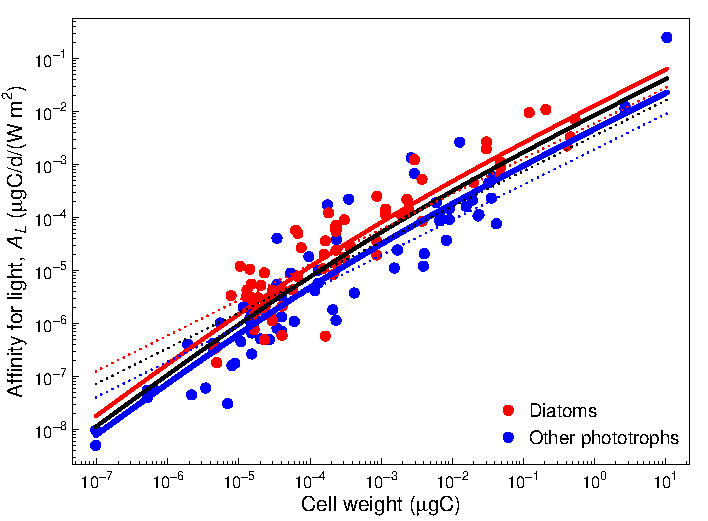
\includegraphics{AL.pdf}
  \caption{Light affinities of protists as a function of carbon mass.  The data are fitted to the self-shading formula (\ref{eq:AL}; thick lines) and to $A_L\propto m^{2/3}$ (dotted lines).  The black lines are fitted to all data.  Data from \citet{Edwards2015}, and conversions from volume to mass is done using the relations in \cite{MendenDeuer2000}.}
  \label{fig:AL}
\end{figure}

\begin{figure}[t]
  \centering
  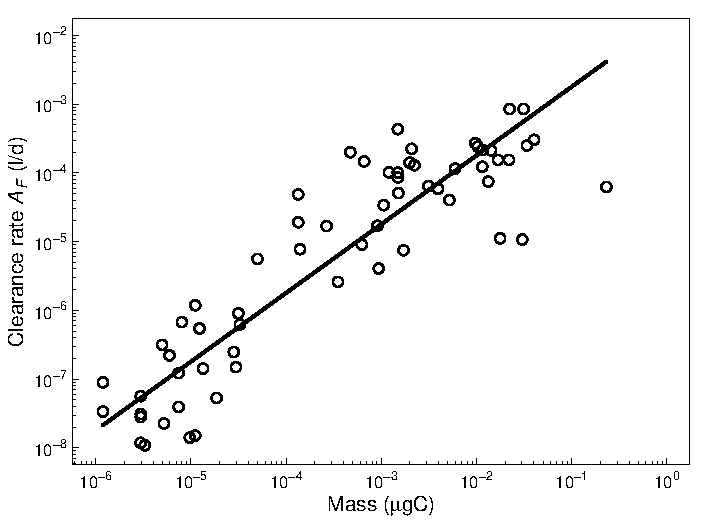
\includegraphics{AF.pdf}
  \caption{Clearance rate ($A_F$) as a function of carbon mass. Data are fitted to $A_F \propto m$. Data of nanoflagellates, dinoflagellates, and ciliates from \citet{Kiorboe2014}.}
  \label{fig:AF}
\end{figure}


\begin{table}[t]
  \centering
  \caption{Parameters.}
  \begin{tabular}{lll}
    Parameter & Value & Source \\
    \hline
    $\alpha_N$\\
    $\alpha_\DOC$ \\
    $\alpha_L$ & 0.0097 $\mug_C/d/(Wm^2)$ & (3)\\
    $\alpha_F$ \\
    $\epsilon_L$ \\
    $\epsilon_F$ \\
    $\rCN$ \\
    $\beta$ \\
    $\sigma$ \\
    $c$ & 0.001 & \citet{Andersen2015} \\
    $N_0$ & 140 $\mug$ N/l & \\
    $r_\POM$ \\
    $\epsilon_r$ \\
    $d$ \\
    $d_\POM$ \\
    \hline
    %\multicolumn{3}{l}{(3) \citet{Taguchi1976); Fig.~\ref{fig:AL}}
    \hline
  \end{tabular}
  \label{tab:parameters}
\end{table}

\section{Model analysis}

\subsection{Smallest size}
The smallest cell is limited by the cell wall \citep{Raven1994}.  The size where the entire cell is used by the wall is when the wall fraction $\nu = 1$ (\ref{eq:nu}).  That happens at a size:
\begin{equation}
  \label{eq:12}
  m_\mathrm{min} =  \approx \mathrm{\mu g}.
\end{equation}


\subsection*{$R^*$}
\begin{figure}[t]
  \centering
  \includegraphics{Rstar.pdf}
  \caption{Limiting concentrations (``$R^*$'''s) of dissolved nutrients (blue), organic carbon (magenta), and light (green).  Shown for a mortality of $\mu = 0.4$ yr$^{-1}$.}
  \label{fig:Rstar}
\end{figure}

The concentration of limiting resources will be controlled by the size group with the smallest requirement for the resource -- the ``$R^*$'' value, \emph{sensu} \citet{Tilman1982}.  The two limiting resources are the dissolved nutrients and the carbon (DOC).  The limiting concentrations are determined by the equilibrium values of each resource:
\begin{eqnarray}
  \label{eq:Rstar}
  0 &=& \frac{\Jmax}{m} \frac{A_N N^* \rCN }{A_N N^* \rCN + \Jmax} - \mu \\ 
  0 &=& \frac{\Jmax}{m} \frac{A_\DOC X_\DOC^* }{A_\DOC X_\DOC^* + \Jmax} - \mu \\
  0 &=& \frac{\Jmax}{m} \frac{A_L L^* }{A_L L^* + \Jmax} - \mu, \\
\end{eqnarray}
with the affinities given by (\ref{eq:AN}) and (\ref{eq:AL})eq.  Inserting the affinities and $\Jmax$ from (\ref{eq:Jmax}) gives the limiting resource concentrations:
\begin{eqnarray}
  \label{eq:Rstars}
  N^*  &=& m^{2/3} \frac{\alpha_\mathrm{max}}{\alpha_N \rCN} \frac{\mu(1-\nu(m))}{\alpha_\mathrm{max} (1-\nu(m)) - \mu} \\
  X_\DOC^* &=& m^{2/3} \frac{\alpha_\mathrm{max}}{\alpha_\DOC } \frac{\mu(1-\nu(m))}{\alpha_\mathrm{max} (1-\nu(m)) - \mu} \\
  L^* &=& m^{1/3} \frac{\alpha_\mathrm{max}}{\alpha_L } \frac{\mu)}{\alpha_\mathrm{max} (1-\nu(m)) - \mu} 
\end{eqnarray}

Clearly, the limiting concentrations are determined by the smallest
cells, the bacterioplankton (Fig.~\ref{fig:Rstar}).

\subsection{Structure and biomass}
The upper part of the size spectrum is dominated by predator-prey interactions. For this part, we can use size-spectrum theory to calculate the expected solution \citep{Andersen2006b}:
\begin{equation}
  b(m) \propto m^{-1-q+n},
\end{equation}
where $b(m)$ is the biomass spectrum (units of biomass per mass), and $q$ and $n$ are the exponents of the clearance rate and the maximum consumption rate. With $q=n=1$, we find that $b(m) \propto m^{-1}$.  The biomass in each size class is $B(m) \approx b(m)\Delta m$.  The width of the size classes are proportional to the mass itself, $\Delta m = c m$, so we find that the biomass in each bin is constant: a perfect Sheldon spectrum.


We can calculate expected N-level from the N*.  We can then calculate new production.  We can also calculate biomass levels as F*.  Then mortality levels comes from production, and then we have the level of biomass.


\subsection{Higher trophic level mortality}
We can calculate the mortality by higher trophic levels by assuming a Sheldon spectrum, as derived above.  The mortality is \citep{Hartvig2011}:
\begin{equation}
  \mu_p(m_p) = \int \phi(m, m_p) (1-f(m)) A_F(m) b(m)/m\, \mathrm{d}m,
\end{equation}
where the feeding level $f(m)$ is the consumption relative to maximum consumption.  Assuming this to be independent of size, $f(m) = f_0$, we can write the mortality as:
\begin{eqnarray}
  \mu_p(m_p) &=& B_\mathrm{Sheldon}  \frac{1-f_0}{c\,\alpha_F} \int \phi(m, m_p) m^{-1}\, dm \\
  &=& B_\mathrm{Sheldon} \frac{ 1-f_0}{c\,\alpha_F} \sqrt{2 \pi} \beta \sigma e^{\sigma^2/2},
\end{eqnarray}
assuming that $\nu = 0$.  We then see that the mortality is approximately proportional to the level of the spectrum $B_\mathrm{Sheldon}$. 


\bibliographystyle{chicago} 
\bibliography{../../Literature/Bibliography}

\end{document}
